\documentclass{beamer}

\usetheme{PaloAlto}
\usepackage{listings}
\definecolor{azulUC3M}{RGB}{0,6,124}
\definecolor{rojoUC3M}{RGB}{186,50,50}
\definecolor{verdeUC3M}{RGB}{86,204,86}
\definecolor{white}{RGB}{255,255,255}
\definecolor{gray97}{gray}{.97}
\definecolor{gray90}{gray}{.90}
\definecolor{gray75}{gray}{.75}
\definecolor{gray45}{gray}{.45}
\lstset{ frame=Ltb,
     framerule=0pt,
     %aboveskip=0.5cm,
     framextopmargin=3pt,
     framexbottommargin=3pt,
     framexleftmargin=0.2cm,
     % xrightmargin=0.7cm,
     % xleftmargin=0.5cm,
     belowcaptionskip=0.5cm,
     framesep=0pt,
     rulesep=0.2pt,
     backgroundcolor=\color{gray97},
     rulesepcolor=\color{black},
     %
     stringstyle=\ttfamily,
     showstringspaces = false,
     basicstyle=\fontsize{7pt}{9pt}\ttfamily,
     commentstyle=\color{gray45},
     keywordstyle=\bfseries,
     %
     breaklines=true,
     literate= {<lambda>}{$\lambda$}1 {²}{{\textsuperscript{2}}}1 {µ}{$\upmu$}1
   }

   \lstdefinestyle{haskell}{
     language=Haskell,
   }

\usepackage[utf8]{inputenc}
\graphicspath{{../thesis/img/}}

%Information to be included in the title page:
\title[Agis: Search in Haskell]{Agis: Heuristic Search Library in Haskell}
\author[Diego Vicente]{Diego Vicente Martín}
\institute{Universidad Carlos III de Madrid}
\date{October 16th, 2017}

\logo{
\includegraphics[height=1.2cm]{slides-logo.png}}

\begin{document}

\frame{\titlepage}

\begin{frame}
  \frametitle{Motivation}
  Why?
  \begin{itemize}
  \item Concurrency/Parallelism is \textbf{hard}.
  \item Haskell provides a clean, minimal syntax.
  \item Functional programming is adequate for search.
  \item There is nothing like this already developed.
  \end{itemize}
\end{frame}

\begin{frame}
  \frametitle{Objectives}
  Develop a complete framework to work with heuristic search problems and
  research in Haskell, containing:
  \begin{itemize}
  \item A search algorithms library.
  \item Predefined search domains.
  \item Benchmark suites and tools.
  \item Full API documentation with examples.
  \end{itemize}
\end{frame}

\begin{frame}[fragile]
  \frametitle{Purity and $k$ Shortest Paths}
  \begin{itemize}
  \item It is not easy to translate typical pseudo-code to pure functional
    paradigm: no loops, no variables, no general state...
  \item Ideally, the output of functions should depend on its input only.
  \item This can be achieved by including a closed list per node.
  \item Inherently using infinite data structures let us solve the $k$ shortest
    paths problem as well as regular searches.
  \end{itemize}

\begin{lstlisting}[style=haskell]
sols = bfs problem  -- infinite list of solutions
print $ head sols   -- computes the first solution
print $ take 5 sols -- computes 5 first solutions
\end{lstlisting}
\end{frame}


\begin{frame}
  \frametitle{Use Cases}
  \begin{itemize}
  \item Solve a search problem.
  \item Get search statistics.
  \item Design a new search algorithm.
  \item Test a search algorithm.
  \item Benchmark a search algorithm.
  \end{itemize}
\end{frame}

\begin{frame}
  \frametitle{Project Artifacts}
  \begin{itemize}
  \item 28 functional requirements.
  \item 4 non-functional requirements.
  \item 2 \emph{type-signature graph} for visual intuition.
  \end{itemize}
\end{frame}

\begin{frame}
  \frametitle{Type-Signature Graphs}
  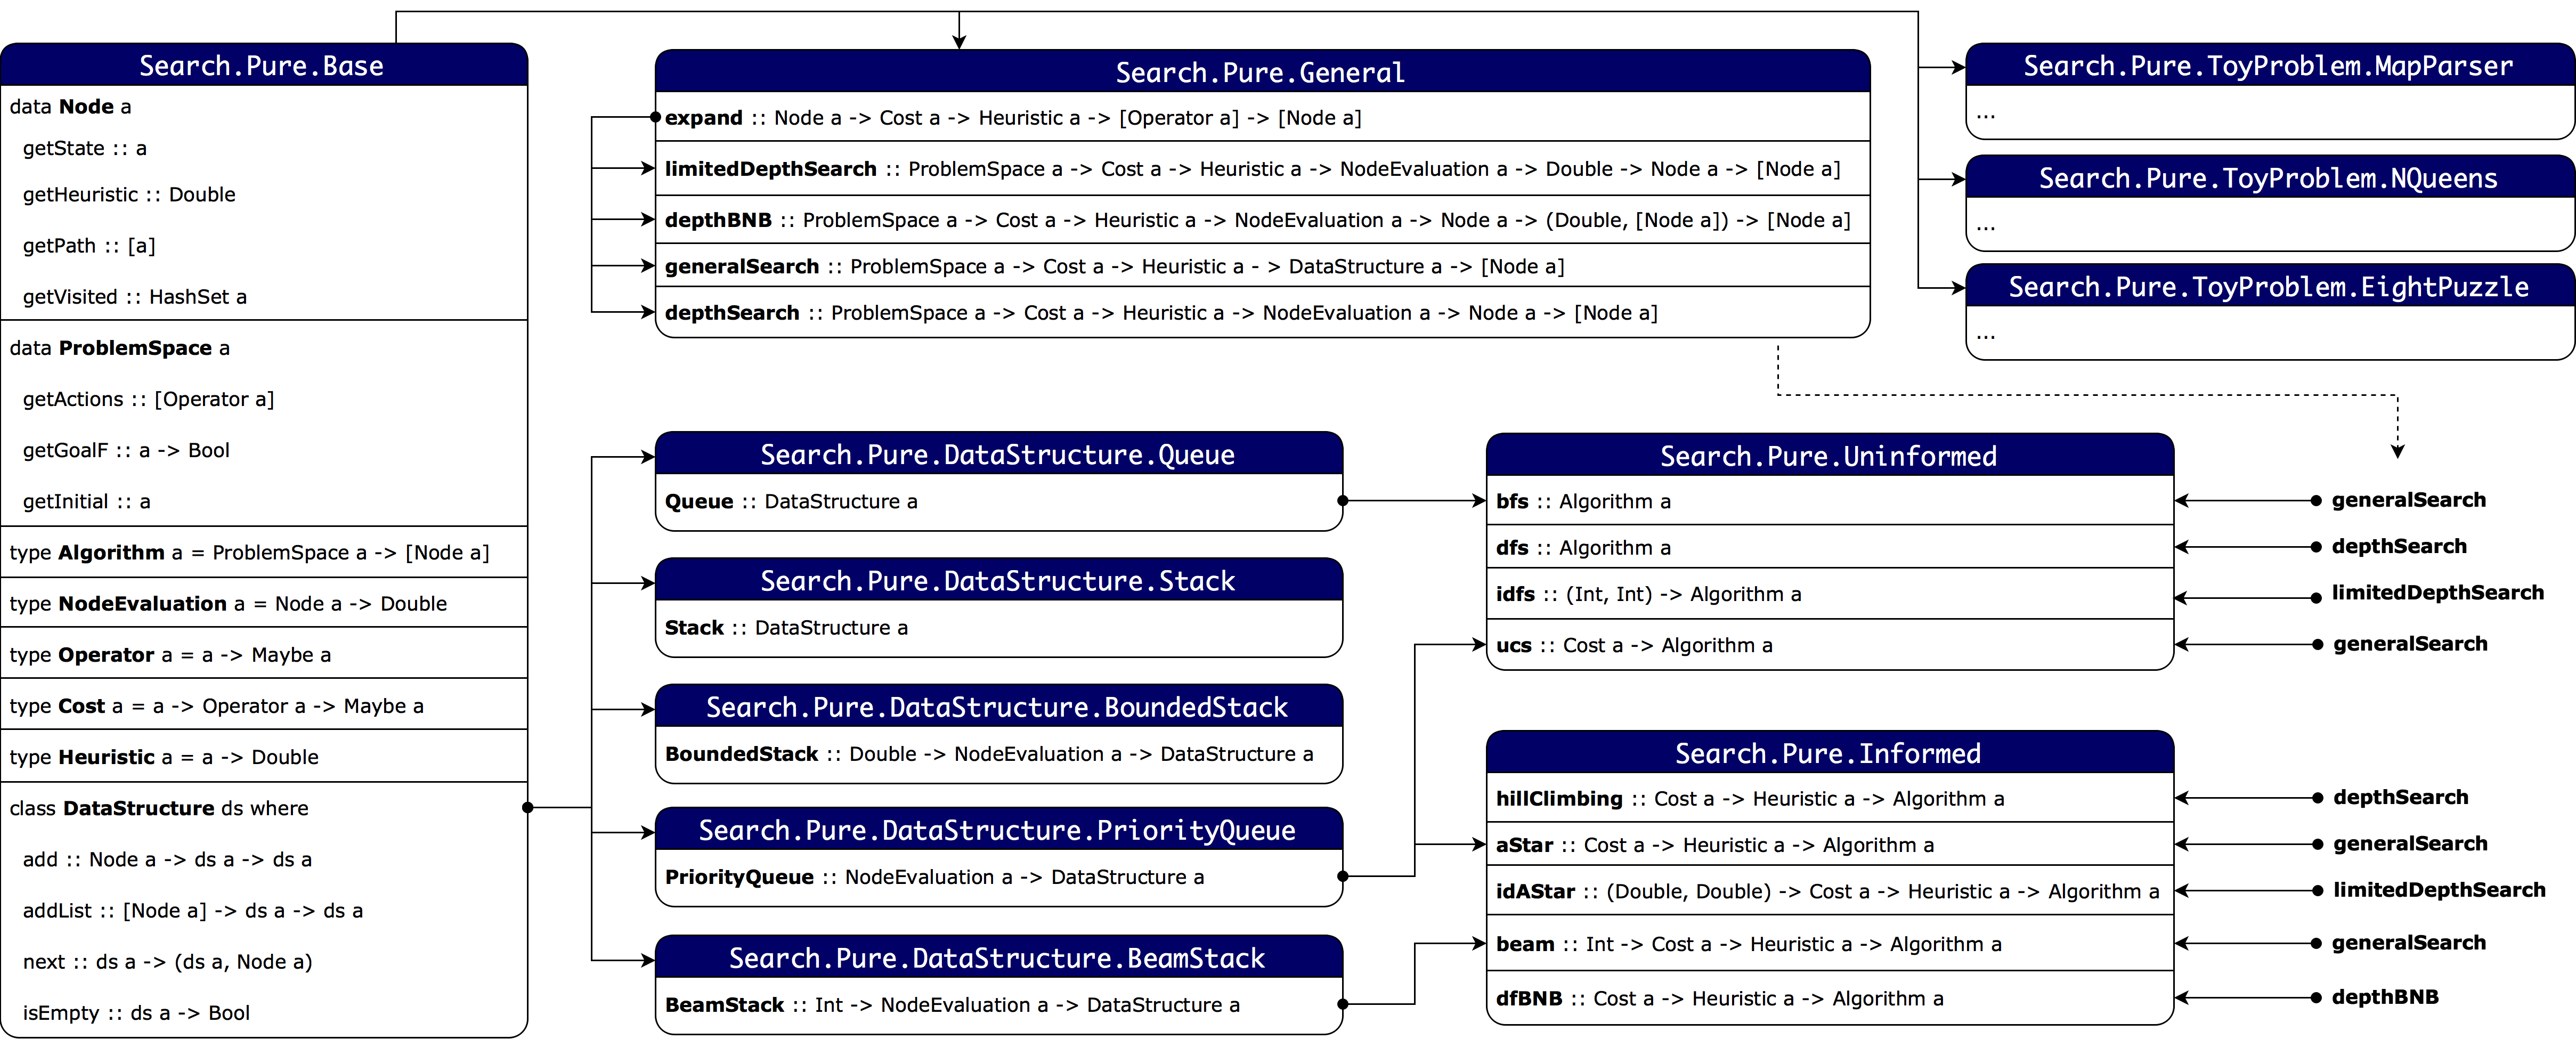
\includegraphics[width=\textwidth]{type-graph-pure.png}
\end{frame}

\begin{frame}
  \frametitle{General Search Implementation}
  A primitive general search is inspired in Russel and Norvig's
  \emph{Artificial Intelligence: A Modern Approach} algorithm
  \texttt{GENERAL\_SEARCH}:
  \begin{itemize}
  \item Uses a data structure to store expanded nodes.
  \item Asks the structure for a node, checks it, expands it, stores the
    resulting nodes in the structure again.
  \item The algorithm's behavior is defined by the data structure.
  \end{itemize}
\end{frame}

\begin{frame}[fragile]
  \frametitle{General Search Implementation}
\begin{lstlisting}[style=haskell]
generalSearch :: (DataStructure ds, Eq a, Hashable a)
  => ProblemSpace a
  -- ^ 'ProblemSpace' to be solved
  -> Cost a
  -- ^ 'Cost' function to use
  -> Heuristic a
  -- ^ 'Heuristic' function to use
  -> ds a
  -- ^ 'DataStructure' that manages the node expansion
  -> [Node a]
  -- ^ Returns the list of all final nodes (solutions)

generalSearch problem g h nodes
  | isEmpty nodes = []
  | getGoalF problem (getState n) =
    n : generalSearch problem g h nodes'
  | otherwise = generalSearch problem g h ds'

  where (nodes', n) = next nodes
        expanded = expand n g h (getActions p)
        ds' = addList expanded nodes'
\end{lstlisting}
\end{frame}

\begin{frame}
  \frametitle{Linear-Memory Search Implementation}
  Many algorithms require linear-memory cost to be valid primitives.
  \begin{itemize}
  \item Use \texttt{map} and recursion to expand the nodes.
  \item General depth-first behavior, can be changed by the functions passed to
    it.
  \item Use of \texttt{map} is cheap and enables high-level concurrent
    abstractions.
  \item Alternative version can receive a node evaluation function and a limit
    to perform bounded depth-first search.
  \end{itemize}
\end{frame}

\begin{frame}[fragile]
  \frametitle{Linear-Memory Implementation}
\begin{lstlisting}[style=haskell]
depthSearch :: (Eq a, Hashable a)
  => ProblemSpace a
  -- ^ 'ProblemSpace' to be solved
  -> Cost a
  -- ^ 'Cost' function to use
  -> Heuristic a
  -- ^ 'Heuristic' function to use
  -> NodeEvaluation a
  -- ^ 'NodeEvaluation' to sort the expanded nodes
  -> Node a
  -- ^ Current 'Node' to be expanded
  -> [Node a]
  -- ^ Returns the list of all solutions

depthSearch problem g h f node
  | getGoalF problem (getState node) = return node
  | otherwise = concatMap (depthSearch problem g h f) sorted
    where sorted = sortBy (\n n' -> compare (f n) (f n')) ns
          ns = expand node g h (getActions problem)
\end{lstlisting}
\end{frame}

\begin{frame}
  \frametitle{Branch and Bound Search Implementation}
  Another primitive to use is a general Branch and Bound search:
  \begin{itemize}
  \item Branch and Bound algorithms uses the best solution found cost as
    current bound; then keeps expanding the tree with new solutions.
  \item Use a \texttt{fold} to traverse the tree with the best solution and
    current bound until search space is exhausted.
  \item Does not find the best $k$ solutions.
  \end{itemize}
  \centering
  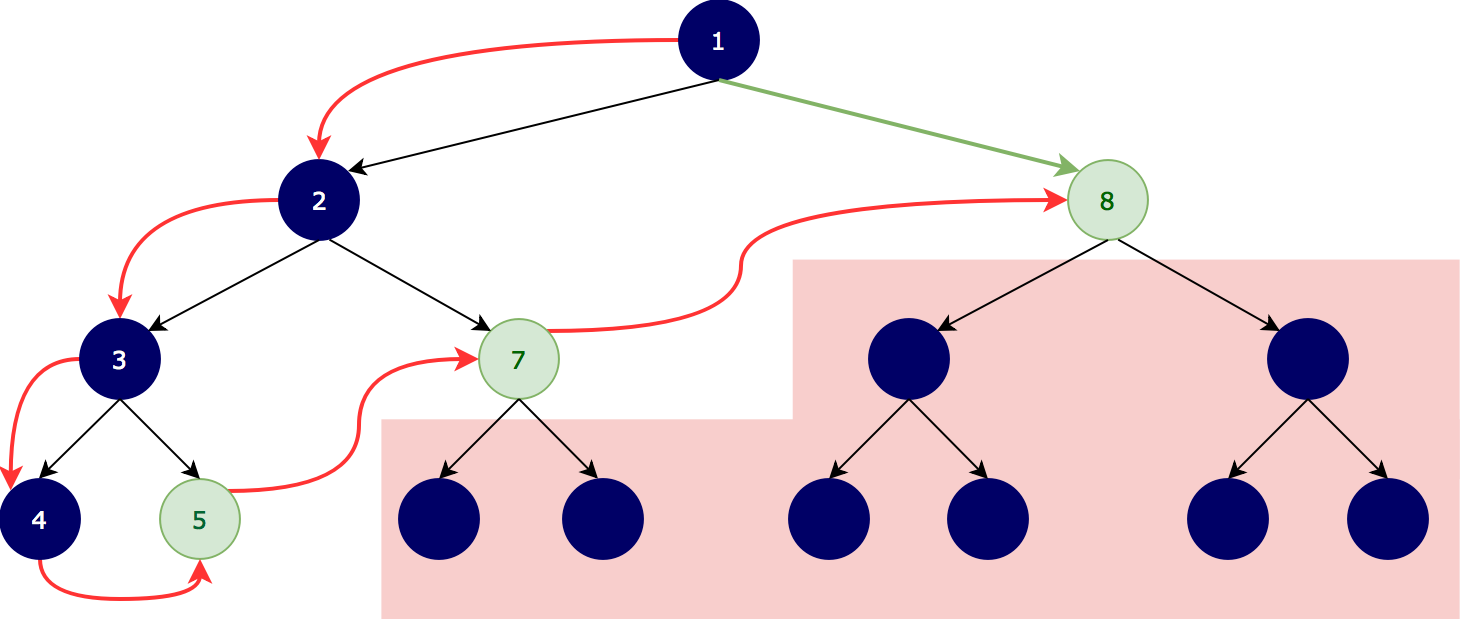
\includegraphics[width=0.7\textwidth]{dfbnb.png}
\end{frame}

\begin{frame}[fragile]
  \frametitle{Branch and Bound Implementation}
\begin{lstlisting}[style=haskell]
depthBNB :: (Eq a, Hashable a)
  => ProblemSpace a
  -- ^ 'ProblemSpace' to be solved
  -> Cost a
  -- ^ 'Cost' function to use
  -> Heuristic a
  -- ^ 'Heuristic' function to use
  -> NodeEvaluation a
  -- ^ 'NodeEvaluation' to sort and bound the expanded nodes
  -> Node a
  -- ^ Current 'Node' to be expanded
  -> (Double, [Node a])
  -- ^ The current bound and intermediate solutions found
  -> (Double, [Node a])
  -- ^ The final bound and all solutions found
depthBNB problem g h f n (l, sol) = foldl bnbStep (l, sol) sorted
  where sorted = sortBy (\n n' -> compare (f n) (f n')) expanded
        expanded = expand n g h (getActions problem)
        bnbStep (bound, solutions) n
          | f n >= bound = (bound, solutions)
          | getGoalF problem (getState n) = (f n, n:solutions)
          | otherwise = depthBNB problem g h f n (bound, solutions)
\end{lstlisting}
\end{frame}


\end{document}





%%% Local Variables:
%%% mode: latex
%%% TeX-master: t
%%% End:
